\chapter{INSTALASI QGIS}

Cara instalasi aplikasi QGIS berbeda antara menggunakan sistem operasi Windows dan sistem operasi Linux.

\begin{enumerate}[A.]

\item Instalasi QGIS di lingkungan Sistem Operasi Windows

Untuk sistem operasi Windows, perangkat lunak QGIS dapat di unduh secara gratis di \textit{website} resmi QuantumGIS dengan alamat http://qgis.org/ melalui berbagai macam \textit{web browser} seperti Firefox, Chrome, Opera, atau Internet Explorer. Tahapannya adalah sebagai berikut :

\begin{enumerate}[1.]

\item Pada kolom halaman di atas jendela \textit{browser}, masukan teks berikut dan tekan Enter : http://qgis.org/, sehingga muncul jendela pada gambar \ref{fig:qgishomepage} :

\begin{figure}
  \centering
  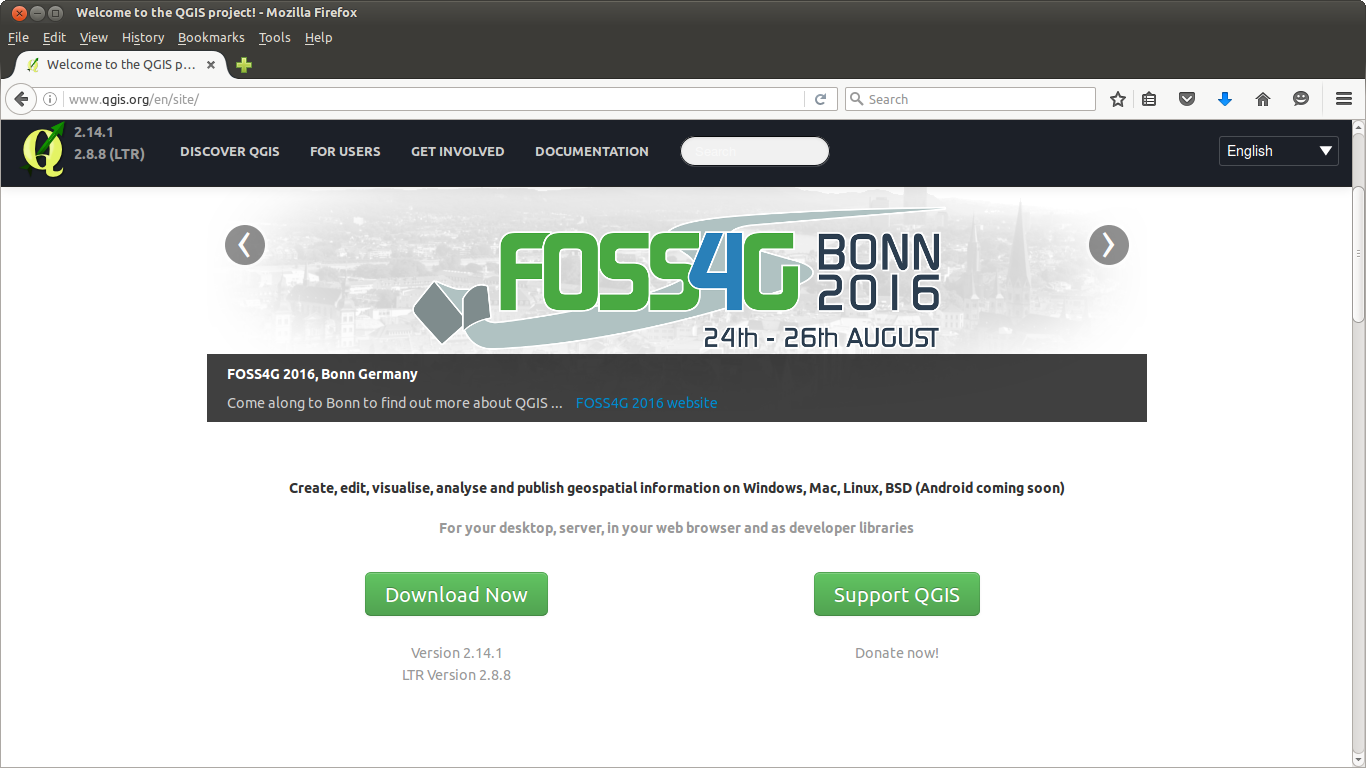
\includegraphics[width=1\textwidth]{./resources/001-homepage-qgis}
  \caption{Jendela \textit{website} QGIS}
  \label{fig:qgishomepage}
\end{figure}

\item Klik \verb|Download Now| pada halaman tersebut.

\item Pada jendela \textit{download} seperti ditampilkan dalam gambar \ref{fig:qgisversion} akan terdapat pilihan QGIS \textit{installer} berdasarkan sistem operasi perangkat yang anda gunakan. \textit{Expand} pilihan sistem operasi yang anda gunakan, lalu klik pada \textbf{Standalone Installer} (direkomendasikan untuk pengguna pemula).

\begin{figure}
  \centering
  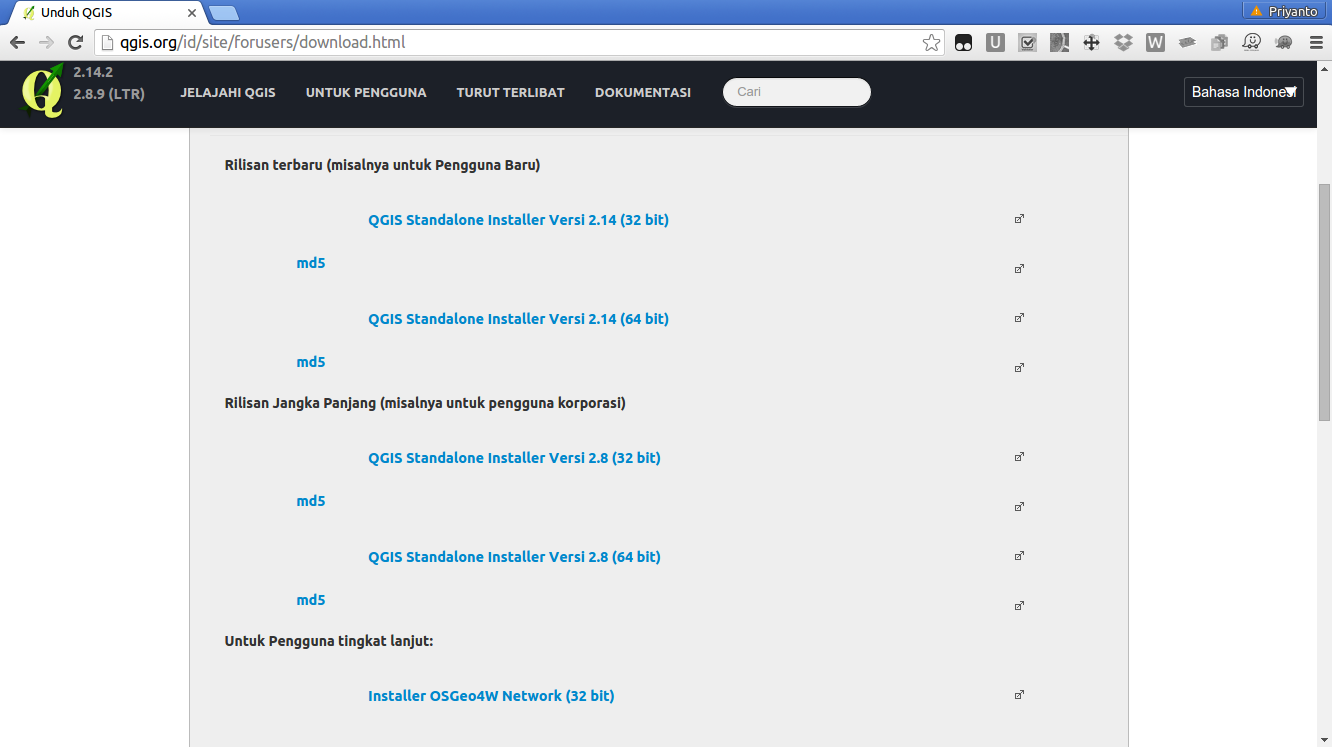
\includegraphics[width=1\textwidth]{./resources/002-pilihan-versi}
  \caption{Pilihan Versi QGIS}
  \label{fig:qgisversion}
\end{figure}

\item Apabila QGIS telah berhasil diunduh, cari \textit{file} instalasi pada direktori yang telah anda tentukan sebelumnya.

\item Klik dua kali pada \textit{file} instalasi tersebut untuk memulai penginstalan QGIS.

\end{enumerate}

\item Instalasi QGIS di lingkungan Sistem Operasi Linux (Debian/Ubuntu)

Instalasi QGIS di lingkungan sistem operasi linux berbeda-beda untuk setiap distro, pada pembahasan kali ini akan diuraikan dengan menggunakan distro dari keluarga Debian, yaitu Ubuntu.

\begin{enumerate}[1.]

\item Langkah pertamanya adalah mengubah isi dari \textit{file} \verb|/etc/apt/sources.list| agar Ubuntu dapat memahami dimana letak repositori QGIS berada. Isikan pada bagian paling bawah saja dengan baris kode berikut :

\begin{verbatim}
deb  http://qgis.org/debian trusty main
\end{verbatim}

atau 

\begin{verbatim}
\end{verbatim}

\end{enumerate}

\end{enumerate}